\documentclass{article}

\usepackage[utf8]{inputenc}
\usepackage[T1]{fontenc}
\usepackage{amsmath}
\usepackage{amsfonts}
\usepackage{amssymb}
\usepackage[version=4]{mhchem}
\usepackage{stmaryrd}
\usepackage{bbold}
\usepackage{graphicx}
\usepackage{adjustbox}
\usepackage{tocloft}   % For TOC formatting
\usepackage{geometry}  % For margins
\usepackage{titlesec}  % For section formatting
\usepackage{fancyhdr}
\usepackage{float}
\usepackage[stable]{footmisc}
\usepackage{hyperref}  % For clickable links in TOC (load last)
\usepackage{mdframed}  
\usepackage{listings}  



% Document styling
\geometry{margin=1in}

% Customize section formatting (option 2: let titlesec handle the label)
\titleformat{\section}
  {\normalfont\Large\bfseries} % format
  {\thesection}                % label
  {0.5em}                      % separation
  {\rule{\textwidth}{0.4pt}\vspace{0.5em}\newline} % before-code

% adding a header
\pagestyle{fancy}
\fancyhf{}
\lhead{Problem Set 2}
\rhead{Henrik Berger - Romain Fernex}
\cfoot{ \thepage}
\renewcommand{\headrulewidth}{0.8pt}

\title{Problem Set 2 - Macroeconomics}
\author{Henrik Berger - Romain Fernex}
\date{February 2025}

\begin{document}

\maketitle
\tableofcontents
\newpage

\section{Literature review}

\begin{figure}[H]
    \centering
    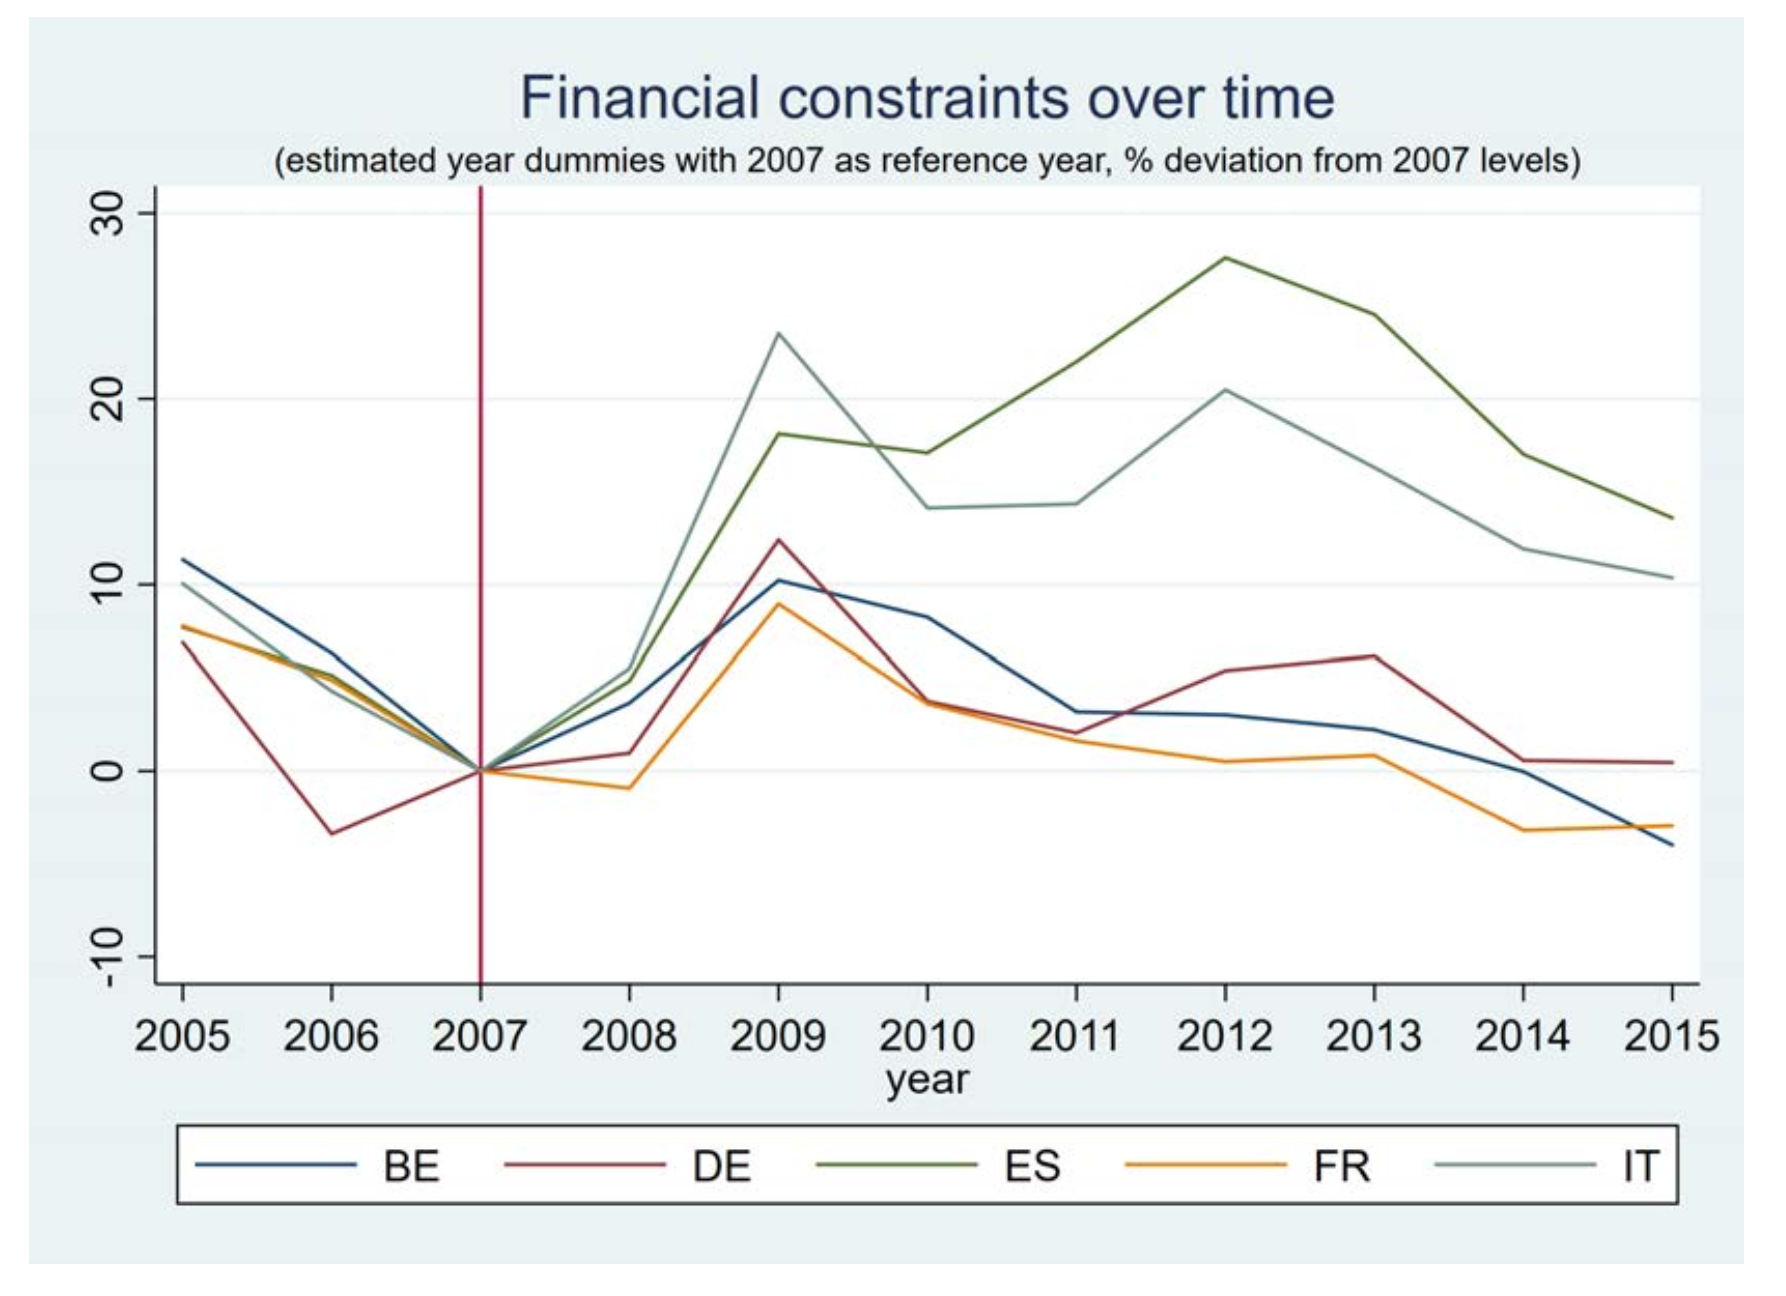
\includegraphics[width=0.8\textwidth]{figures/Screenshot 2025-10-11 at 8.09.59 PM.png}
    \caption{Financial constraints over time}
    \label{fig: financial constraints over time}
\end{figure}
The authors construct their financial constraint metric by comparing firms’ observed input–output choices to a nonparametric production frontier that represents optimal behavior under full access to finance. The distance from this frontier captures how far each firm operates below its unconstrained potential, interpreted as a shadow cost of external finance. They then classify firms into “mildly,” “moderately,” or “strongly” constrained categories using cutoffs on this latent measure.

Figure 3 plots, for major EU countries between 2005 and 2015, the average share of firms identified as constrained. The graph reveals pronounced cross-country heterogeneity: Italy and Spain show a sharp rise in constraint incidence during the Great Recession and Eurozone crisis, while Germany and France maintain lower, flatter trajectories. The common to all four upward movements in crisis years and the slow recovery afterward suggest that the measure captures persistent financial stress rather than short-term volatility.

Overall, the figure provides a clear empirical picture of the uneven distribution of financial frictions within a common monetary framework. It demonstrates that the latent frontier-based indicator generates plausible temporal and cross-sectional patterns consistent with major financial disruptions, and that its stability and coherence make it a credible empirical proxy for firm-level financial constraints.


\section{Exercise I}

\subsection{Part A}

\subsubsection{1)}
Entrepreneurs wish to maximize their profits $\pi_t$ as this is what they consume. It is defined as follows : 
$$c_{e,t}=\pi_t = y_t-(1+r_t)k_{t} = k_t^\alpha -(1+r_t)k_{t}$$
We maximze profits with respect to $k_t$ and get : 
$$\alpha k_t^{\alpha-1}=1+r$$
In steady state the time indexes disappear and we get : 
$$\alpha k^{\alpha-1}=1+r$$
We can now consume the steady state profits which correspond to $c_{e}$ :
$c_e = \pi = k^{\alpha}-(1+r)k = k^{\alpha}-\alpha k^{\alpha-1}k = (1-\alpha)k^{\alpha}$

\subsubsection{2)}
We have : 
$$c_A + c_B + k + c_e =1+f(k)$$
The right hand side corresponds to the aggregate wealth available in each period. It combines both the wealth produced by the entrepreneur and the combined endowment of agent A and B (which always sums to 1) in a given period. This wealth is then consumed by each of the agent or invested in production. It is worth noting that capital loan repayments are just a transfer of wealth so it does not appear as it is zero sum. 

\subsection{Part B}

\subsubsection{1)}
\textbf{a,b,c)}
The optimization programm of the rich agent is as follows : 
$$\begin{aligned}
    \max_{a_{t+1}^R}& \quad u(c_t^R)+\beta u((1+r_{t+1})a^R_{t+1}-a_{t+2}^P)\\
    \text{s.t }\quad &\text{budget constraint : } c_t^R = (1+r_t)a^P_t-a_{t+1}^R+1\\
    &\text{borrowing constraint : } a_{t+1}^R  \geq 0
\end{aligned}$$
Using two period notation this gives : 
$$\begin{aligned}
    \max_{a'^R}& \quad u(c^R)+\beta u((1+r')a'^R-a''^P)\\
    \text{s.t }\quad &\text{budget constraint : } c^R = (1+r)a^P-a'^R+1\\
    &\text{borrowing constraint : } a'^R \geq 0
\end{aligned}$$
\textbf{d)}
The state variable is $a^P$ and the control variables are $a'^R$ and $c^R$. $r$ is endogenously determined and $e$ (the endowment) can be considered a determined idiosyncratic shock. 
\textbf{e)}
The Bellman equation for this program is as follows : 
$$\begin{aligned}
    V_R(a^P) = &\max_{a'^R}\quad u(c^R)+\beta V_P(a'^R)\\
    \text{s.t} \quad &a'^R \geq  0\\
    &c^R=(1+r)a^P-a'^R+1
\end{aligned} $$
Hence, 
$$V_R(a^P) = \max_{a'^R}\quad u((1+r)a^P-a'^R+1)+\beta V_P(a'^R)$$
\textbf{f)}
We assume the budget constraint does not bind.
\begin{itemize}
    \item step 1 : we get the FOC in $a'^R$
    $$u'(c^R)=\beta V_P'(a'^P)$$
    \item step 2 : we get the envelope condition in $a^P$ : 
    $$V_R'(a^P) = (1+r)u'(c^R)$$
    \item step 3 : we iterate the envelope condition : 
    $$V_R'(a')=(1+r')u'(c'^R)$$
\end{itemize}
\subsubsection{2)}
\textbf{a)}
For the poor, we have the following optimization programm : 
$$\begin{aligned}
    V_P(a^R) = &\max_{a'^P}\quad u(c^P)+\beta V_R(a'^P)\\
    \text{s.t} \quad &a'^P \geq  0\\
    &c^P=(1+r)a^R-a'^P
\end{aligned} $$
\textbf{b)}
We assume the budget constraint does not bind.
\begin{itemize}
    \item step 1 : we get the FOC in $a'^P$
    $$u'(c^P)=\beta V_R'(a'^P)$$
    \item step 2 : we get the envelope condition in $a^R$ : 
    $$V_P'(a^R) = (1+r)u'(c^P)$$
    \item step 3 : we iterate the envelope condition : 
    $$V_P'(a'^R)=(1+r')u'(c'^P)$$
\end{itemize}
\subsubsection{3)}
From the above we get : 
$$\left\{\begin{aligned}
    &u'(c^P)=\beta V_R'(a'^P)\\
    &V_P'(a'^R)=(1+r')u'(c'^P)\\
    &u'(c^R)=\beta V_P'(a'^P)\\
    &V_R'(a')=(1+r')u'(c'^R)
\end{aligned} \right.$$
This gives us the following Euler equations when the borrowing constraint is not binding : 
$$\left\{\begin{aligned}
    &u'(c^P)=\beta (1+r')u'(c'^R)\\
    & u'(c^R)=\beta (1+r')u'(c'^P)
\end{aligned} \right.$$
\subsubsection{4)}
Using the above result at the steady state, we get : 
$$\begin{aligned}
    [u'(c^P)+u'(c^R)] &=\beta (1+r) [u'(c^R)+u'(c^P)]\\
    1 &= \beta(1+r)\\
    \frac{1}{\beta} &= (1+r
\end{aligned}$$
Then we have : 
$$u'(c^P)=u'(c^R)$$
Since u is monotonic increasing it is invertible and we get :
$$c^P=c^R$$

\subsubsection{5)}
Since we have complete market and the borrowing constraints are not binding , the agents can perfectly smooth consumption from one period to the other. Thus this mimics the representative-agent RBC framework and we get the same steady state interest rate $1+r=\frac{1}{\beta}$. Besides there is perfect risk sharing so $c_P=c_R$ which is also in line with what we get from the frictionless RBC model.

\subsubsection{6)}
If this is a lump sum tax then the tax won't affect the intertemporal tradeoff (materialized by the euler equations) and thus will not impact our result for the interest rate. \\
In the case of an ad valorem tax on asset returns, however, it will have an impact and we will get : $$1+r = \frac{1}{\beta(1-T)}$$
The interest rate is higher since the agents A and B will want to compensate for the loss in consumption due to the tax (the marginal utility of consumption in the affected states is higher). 

\subsection{Part C}
\textbf{1)}
The Program of the poor agent : the borrowing constraint binds 
$$\begin{aligned}
    \max_{a_{t+1}^P} &\quad u((1+r_t)a_t^R-a_{t+1}^P)+\beta u((1+r_{t+1})a_{t+1}^P-a_{t+2}^R+1)\\
    \text{s.t} &\quad a_{t+1}^P > 0
\end{aligned}$$
The Program of the rich agent : the borrowing constraint does not  bind !
$$\begin{aligned}
    \max_{a_{t+1}^P} &\quad u((1+r_t)a_t^P-a_{t+1}^R+1)+\beta u((1+r_{t+1})a_{t+1}^R-a_{t+2}^P)
\end{aligned}$$
Solving for the FOC of the rich agent gives us : 
$$u(c_t^R)=(1+r_{t+1})u'(c_{t+1}^P)$$
So in steady state we get : 
$$\frac{u(c^R)}{u(c^P)}=\beta (1+r)$$
Then, using the FOC for the poor agent : we denote $\lambda_t$ the shadow value of the borrowing constraint
$$\begin{aligned}
    u'(c_t^P)=\beta(1+r_{t+1})u'(c_{t+1}^R)+\lambda_t\\
    \Leftrightarrow \frac{u'(c_t^P)}{u(c_{t+1}^R)}-\beta (1+r_{t+1})=\frac{\lambda_t}{u'(c_{t+1}^R)}
\end{aligned}$$
Hence, in steady state : the constraint binds ($\lambda >0$) and $u'>0$
$$\frac{u'(c^P)}{u'(c^R)}-\beta (1+r) = \frac{\lambda}{u(c^R)}>0$$
Thus, 
$$\frac{u'(c^P)}{u'(c^R)} > \beta (1+r)$$

\subsubsection{2)}
1) For the rich agent, we have : the constraint held with equality for the poor (which he was last period) so $a_t^P=0$
$$c_t^R = (1+r)a_t^P+1-a_{t+1}^R=1-a_{t+1}^R$$
In steady state this gives : 
$$c^R=1-a^R$$
2) For the poor agent, we have : the constraint holds with equality for the poor restricting his capacity to borrow now $a_{t+1}^P=0$
$$c_t^P=(1+r_t)a_t^R-a_{t+1}^P$$
In steady state this gives : 
$$c^P = (1+r)a$$
3) Only the rich lends to the entrepreneurs as they are not constrained. Thus the entrepreneurs' only source of capital is what they borrow from the rich agent which is $a^R$ ins stead state. Hence : 
$$a^R=k$$

\subsubsection{3)}
Based on previous questions, with $u(c)=log(c) \Leftrightarrow u'(c)=\frac{1}{c}$
$$\left\{\begin{aligned}
    &\frac{u'(c^R)}{u'(c^P)}=\beta(1+r)  \Leftrightarrow \frac{c^P}{c^R}=\beta(1+r)\\
    &c^R+a^R=1\\
    &c^P = a^R(1+r)\\
    &a^R=k
\end{aligned} \right.$$
This gives : 
$$\begin{aligned}
    \frac{a^R(1+r)}{1-a^R}=\beta(1+r)\\
    \Leftrightarrow \frac{k(1+r)}{1-k}=\beta\\
    \Leftrightarrow \frac{k}{1-k}=\beta\\
    \Leftrightarrow k = \beta -k\beta\\
    \Leftrightarrow k=\frac{\beta}{1+\beta}
\end{aligned}$$

\subsubsection{4)}
We know from part A : $$\alpha k^{\alpha-1}=1+r$$
Combining this with the equality we got in (3) we get : we denote $r_{CC}$ the interest rate with the credit constraint and $r_{NC}$ without 
$$\alpha(\frac{\beta}{1+\beta})^{\alpha-1}=1+r_{CC}\Leftrightarrow\alpha (\frac{1+\beta}\beta{)^{1-\alpha}=1+r_{CC}}$$
We know that without credit constraint we get $1+r_{NC}=\frac{1}{\beta}$. Granted $\alpha,\beta \in (0,1)$ we get : 
$$1+r_{CC}=\alpha (\frac{1+\beta}\beta{)^{1-\alpha}} < \frac{1}{\beta}=1+r_{NC}$$
This difference is due to the fact that the poor agents are now credit constrained. This means rich agents transfer more utility to the next period to compensate for this. This exerts a downward pressure on the interest rate compared the case when they are not credit constrained.  \\
Now let's look at the steady state capital stock : without credit constraints we have
$$\begin{aligned}
    1+r_{NC} &= \alpha k^{\alpha-1}\\
    \Leftrightarrow \frac{1}{\beta}&=\alpha k^{\alpha-1}\\
    \Leftrightarrow (\alpha\beta)^{\frac{1}{1-\alpha}}&=k_{CC}
\end{aligned}$$
So we get : 
$$\left\{\begin{aligned}
    k_{NC}=(\alpha\beta)^{\frac{1}{1-\alpha}}\\
    k_{CC} = \frac{\beta}{1+\beta}
\end{aligned}\right.$$
Written using the interest rate this translates to : 
$$\left\{\begin{aligned}
    k_{NC}=(\frac{\alpha}{1+r_{NC}})^{\frac{1}{1-\alpha}}\\
    k_{CC} =(\frac{\alpha}{1+r_{CC}})^{\frac{1}{1-\alpha}}
\end{aligned}\right.$$
Based on the inequality we established above this means : $\forall \beta,\alpha \in (0,1)$
$$k_{NC}<k_{CC}$$
The steady state capital is larger when the credit constraints bind, this is line with our above statement about capital overaccumulation. The households (agents A and B) can’t move resources from poor to rich states by borrowing. To smooth consumption across states, they save more in the rich state. That extra saving pushes up the supply of capital.

\subsubsection{5)}
If we introduce a lump sum tax in periods where the agent is richer this will push the interest rate upwards. Indeed, the households cannot invest as much as before in the firms due to its diminished wealth and will ask a greater return on the capital lent to the firms to preserve their utility in the periods when they are poor. In other words, the lower rich-state saving reduces capital supplied, which raises the marginal product and hence the interest rate through the firm’s FOC. 

\subsubsection{6)}
The mechanism described in 5) is not present in part B) because the households are not constrained in periods where he gets less endowment. This means they can safely transfer his utility across states and smooth their consumption across states following the impact of the tax. The interest rate thus remains unchanged as the intertemporal tradeoff is not affected compared to the case where the households are constrained and need to compensate for the loss. 

\section{Exercise II}
Please find the associated notebook at the following link :  \href{https://pluto.land/n/5hvn1ssv}{Notebook for Exercise 2} 


\section{Reference}
Ferrando, Annalisa and Mulier, Klaas and Cherchye, Laurens and Rock, Bram De and Verschelde, Marijn, Identifying Financial Constraints (June, 2020). ECB Working Paper No. 20202420
\end{document}


